% Options for packages loaded elsewhere
\PassOptionsToPackage{unicode}{hyperref}
\PassOptionsToPackage{hyphens}{url}
\PassOptionsToPackage{dvipsnames,svgnames,x11names}{xcolor}
%
\documentclass[
  letterpaper,
  DIV=11,
  numbers=noendperiod]{scrartcl}

\usepackage{amsmath,amssymb}
\usepackage{iftex}
\ifPDFTeX
  \usepackage[T1]{fontenc}
  \usepackage[utf8]{inputenc}
  \usepackage{textcomp} % provide euro and other symbols
\else % if luatex or xetex
  \usepackage{unicode-math}
  \defaultfontfeatures{Scale=MatchLowercase}
  \defaultfontfeatures[\rmfamily]{Ligatures=TeX,Scale=1}
\fi
\usepackage{lmodern}
\ifPDFTeX\else  
    % xetex/luatex font selection
\fi
% Use upquote if available, for straight quotes in verbatim environments
\IfFileExists{upquote.sty}{\usepackage{upquote}}{}
\IfFileExists{microtype.sty}{% use microtype if available
  \usepackage[]{microtype}
  \UseMicrotypeSet[protrusion]{basicmath} % disable protrusion for tt fonts
}{}
\makeatletter
\@ifundefined{KOMAClassName}{% if non-KOMA class
  \IfFileExists{parskip.sty}{%
    \usepackage{parskip}
  }{% else
    \setlength{\parindent}{0pt}
    \setlength{\parskip}{6pt plus 2pt minus 1pt}}
}{% if KOMA class
  \KOMAoptions{parskip=half}}
\makeatother
\usepackage{xcolor}
\setlength{\emergencystretch}{3em} % prevent overfull lines
\setcounter{secnumdepth}{5}
% Make \paragraph and \subparagraph free-standing
\makeatletter
\ifx\paragraph\undefined\else
  \let\oldparagraph\paragraph
  \renewcommand{\paragraph}{
    \@ifstar
      \xxxParagraphStar
      \xxxParagraphNoStar
  }
  \newcommand{\xxxParagraphStar}[1]{\oldparagraph*{#1}\mbox{}}
  \newcommand{\xxxParagraphNoStar}[1]{\oldparagraph{#1}\mbox{}}
\fi
\ifx\subparagraph\undefined\else
  \let\oldsubparagraph\subparagraph
  \renewcommand{\subparagraph}{
    \@ifstar
      \xxxSubParagraphStar
      \xxxSubParagraphNoStar
  }
  \newcommand{\xxxSubParagraphStar}[1]{\oldsubparagraph*{#1}\mbox{}}
  \newcommand{\xxxSubParagraphNoStar}[1]{\oldsubparagraph{#1}\mbox{}}
\fi
\makeatother


\providecommand{\tightlist}{%
  \setlength{\itemsep}{0pt}\setlength{\parskip}{0pt}}\usepackage{longtable,booktabs,array}
\usepackage{calc} % for calculating minipage widths
% Correct order of tables after \paragraph or \subparagraph
\usepackage{etoolbox}
\makeatletter
\patchcmd\longtable{\par}{\if@noskipsec\mbox{}\fi\par}{}{}
\makeatother
% Allow footnotes in longtable head/foot
\IfFileExists{footnotehyper.sty}{\usepackage{footnotehyper}}{\usepackage{footnote}}
\makesavenoteenv{longtable}
\usepackage{graphicx}
\makeatletter
\def\maxwidth{\ifdim\Gin@nat@width>\linewidth\linewidth\else\Gin@nat@width\fi}
\def\maxheight{\ifdim\Gin@nat@height>\textheight\textheight\else\Gin@nat@height\fi}
\makeatother
% Scale images if necessary, so that they will not overflow the page
% margins by default, and it is still possible to overwrite the defaults
% using explicit options in \includegraphics[width, height, ...]{}
\setkeys{Gin}{width=\maxwidth,height=\maxheight,keepaspectratio}
% Set default figure placement to htbp
\makeatletter
\def\fps@figure{htbp}
\makeatother
% definitions for citeproc citations
\NewDocumentCommand\citeproctext{}{}
\NewDocumentCommand\citeproc{mm}{%
  \begingroup\def\citeproctext{#2}\cite{#1}\endgroup}
\makeatletter
 % allow citations to break across lines
 \let\@cite@ofmt\@firstofone
 % avoid brackets around text for \cite:
 \def\@biblabel#1{}
 \def\@cite#1#2{{#1\if@tempswa , #2\fi}}
\makeatother
\newlength{\cslhangindent}
\setlength{\cslhangindent}{1.5em}
\newlength{\csllabelwidth}
\setlength{\csllabelwidth}{3em}
\newenvironment{CSLReferences}[2] % #1 hanging-indent, #2 entry-spacing
 {\begin{list}{}{%
  \setlength{\itemindent}{0pt}
  \setlength{\leftmargin}{0pt}
  \setlength{\parsep}{0pt}
  % turn on hanging indent if param 1 is 1
  \ifodd #1
   \setlength{\leftmargin}{\cslhangindent}
   \setlength{\itemindent}{-1\cslhangindent}
  \fi
  % set entry spacing
  \setlength{\itemsep}{#2\baselineskip}}}
 {\end{list}}
\usepackage{calc}
\newcommand{\CSLBlock}[1]{\hfill\break\parbox[t]{\linewidth}{\strut\ignorespaces#1\strut}}
\newcommand{\CSLLeftMargin}[1]{\parbox[t]{\csllabelwidth}{\strut#1\strut}}
\newcommand{\CSLRightInline}[1]{\parbox[t]{\linewidth - \csllabelwidth}{\strut#1\strut}}
\newcommand{\CSLIndent}[1]{\hspace{\cslhangindent}#1}

\usepackage{float}
\usepackage{tabularray}
\usepackage[normalem]{ulem}
\usepackage{graphicx}
\UseTblrLibrary{booktabs}
\UseTblrLibrary{rotating}
\UseTblrLibrary{siunitx}
\NewTableCommand{\tinytableDefineColor}[3]{\definecolor{#1}{#2}{#3}}
\newcommand{\tinytableTabularrayUnderline}[1]{\underline{#1}}
\newcommand{\tinytableTabularrayStrikeout}[1]{\sout{#1}}
\KOMAoption{captions}{tableheading}
\makeatletter
\@ifpackageloaded{caption}{}{\usepackage{caption}}
\AtBeginDocument{%
\ifdefined\contentsname
  \renewcommand*\contentsname{Table of contents}
\else
  \newcommand\contentsname{Table of contents}
\fi
\ifdefined\listfigurename
  \renewcommand*\listfigurename{List of Figures}
\else
  \newcommand\listfigurename{List of Figures}
\fi
\ifdefined\listtablename
  \renewcommand*\listtablename{List of Tables}
\else
  \newcommand\listtablename{List of Tables}
\fi
\ifdefined\figurename
  \renewcommand*\figurename{Figure}
\else
  \newcommand\figurename{Figure}
\fi
\ifdefined\tablename
  \renewcommand*\tablename{Table}
\else
  \newcommand\tablename{Table}
\fi
}
\@ifpackageloaded{float}{}{\usepackage{float}}
\floatstyle{ruled}
\@ifundefined{c@chapter}{\newfloat{codelisting}{h}{lop}}{\newfloat{codelisting}{h}{lop}[chapter]}
\floatname{codelisting}{Listing}
\newcommand*\listoflistings{\listof{codelisting}{List of Listings}}
\makeatother
\makeatletter
\makeatother
\makeatletter
\@ifpackageloaded{caption}{}{\usepackage{caption}}
\@ifpackageloaded{subcaption}{}{\usepackage{subcaption}}
\makeatother

\ifLuaTeX
  \usepackage{selnolig}  % disable illegal ligatures
\fi
\usepackage{bookmark}

\IfFileExists{xurl.sty}{\usepackage{xurl}}{} % add URL line breaks if available
\urlstyle{same} % disable monospaced font for URLs
\hypersetup{
  pdftitle={Are Ambrosia Apples Really on Sale? A Price Comparison Between Loblaws and NoFrills},
  pdfauthor={Viet Nguyen; Yihang Xu; Doran Wang},
  colorlinks=true,
  linkcolor={blue},
  filecolor={Maroon},
  citecolor={Blue},
  urlcolor={Blue},
  pdfcreator={LaTeX via pandoc}}


\title{Are Ambrosia Apples Really on Sale? A Price Comparison Between
Loblaws and NoFrills\thanks{Code and data are available at:}}
\author{Viet Nguyen \and Yihang Xu \and Doran Wang}
\date{November 14, 2024}

\begin{document}
\maketitle
\begin{abstract}
This study investigates the pricing of Ambrosia apples at two major
grocery retailers, Loblaws and NoFrills, to determine the validity of
advertised sales. Loblaws claims to offer Ambrosia apples at a
discounted price of \$1.21 per unit, reduced from an original price of
\$1.45. However, a comparison with NoFrills shows that the price of
Ambrosia apples is consistently \$1.21, without any mention of a sale.
This suggests that Loblaws' `sale' may not represent a true discount but
rather a temporary reduction to match NoFrills' regular pricing. These
findings raise questions about the transparency of sale promotions and
highlight the need for consumers to be vigilant when comparing prices.
\end{abstract}

\renewcommand*\contentsname{Table of Contents}
{
\hypersetup{linkcolor=}
\setcounter{tocdepth}{3}
\tableofcontents
}

\section{Introduction}\label{introduction}

Retailers frequently promote products as being ``on sale'' to attract
consumers. However, these promotions may not always represent a genuine
discount. This paper investigates the pricing of Ambrosia apples at two
major Canadian grocery chains, Loblaws and NoFrills. Specifically,
Loblaws advertises a sale price of \$1.21 per unit, reduced from an
original price of \$1.45. Meanwhile, NoFrills consistently offers the
same apples at \$1.21, without labeling it as a sale. This study
explores whether Loblaws' claimed discount reflects an actual price
reduction or simply aligns with competitors' regular prices, raising
questions about pricing transparency.The primary objective of this study
is to evaluate whether Loblaws' advertised sale price on Ambrosia apples
represents a genuine discount. We estimate the validity of this sale by
comparing prices across two vendors---Loblaws and NoFrills---and
investigating if the ``original'' price at Loblaws was artificially
inflated before the sale. The key estimand is the difference between the
regular price and the sale price, considering NoFrills' stable pricing
as a benchmark.Our analysis shows that Loblaws' sale price of \$1.21 for
Ambrosia apples is identical to the regular price at NoFrills, where the
apples are consistently sold at \$1.21 without any indication of a
discount. This finding suggests that Loblaws' ``sale'' does not
represent a true markdown but rather an adjustment to match a
competitor's standard pricing. The original price of \$1.45 at Loblaws
may have been artificially inflated, making the sale appear more
substantial than it is.This research highlights a potential issue of
misleading sales tactics in the retail industry. When consumers believe
they are receiving a discount, they are more likely to purchase, even if
the price is not genuinely lower. Such practices can erode consumer
trust and create unfair competition. Understanding these pricing
dynamics helps consumers make informed decisions and prompts retailers
to adopt more transparent pricing strategies.The remainder of this paper
is structured as follows. In Section~\ref{sec-data}, we provide a
detailed description of the data and methods used for price comparisons.
\textbf{?@sec-result} presents our results, followed by a discussion of
the implications in \textbf{?@sec-discussion}. Finally,
\textbf{?@sec-suggest} offers concluding remarks and suggests directions
for future research.

\section{Data}\label{sec-data}

\subsection{Overview}\label{overview}

We use the statistical programming language R (R Core Team 2023)\ldots.
The data used in this paper came from the (\textbf{hammer?}). Following
Alexander (2023), we considerto capture the pricing dynamics of Ambrosia
apples across different vendors, we extracted relevant data from a
larger dataset containing multiple products and vendors. The initial
dataset included information from seven vendors, each offering various
products. Our focus was on the specific product, ``Ambrosia Apples,''
which was sold by two vendors---NoFrills and Loblaws.From this
comprehensive dataset, we filtered out all other products, isolating
only the entries related to Ambrosia apples. The extracted data included
key information such as the product ID, product name, current price, and
old price. Additionally, a field labeled ``other'' contained further
notes on sale conditions or discounts. The dataset also recorded
timestamps, allowing us to track pricing changes over time.

\subsection{Measurement}\label{measurement}

\begin{longtable}[]{@{}
  >{\raggedright\arraybackslash}p{(\columnwidth - 8\tabcolsep) * \real{0.1720}}
  >{\raggedright\arraybackslash}p{(\columnwidth - 8\tabcolsep) * \real{0.1613}}
  >{\raggedleft\arraybackslash}p{(\columnwidth - 8\tabcolsep) * \real{0.2473}}
  >{\raggedleft\arraybackslash}p{(\columnwidth - 8\tabcolsep) * \real{0.2043}}
  >{\raggedright\arraybackslash}p{(\columnwidth - 8\tabcolsep) * \real{0.2151}}@{}}

\caption{\label{tbl-loblaws_data}Ambrosia Apples Data of Loblaws}

\tabularnewline

\toprule\noalign{}
\begin{minipage}[b]{\linewidth}\raggedright
Product Name
\end{minipage} & \begin{minipage}[b]{\linewidth}\raggedright
Product Vendor
\end{minipage} & \begin{minipage}[b]{\linewidth}\raggedleft
Product Price(current)
\end{minipage} & \begin{minipage}[b]{\linewidth}\raggedleft
Product Price(old)
\end{minipage} & \begin{minipage}[b]{\linewidth}\raggedright
Date
\end{minipage} \\
\midrule\noalign{}
\endhead
\bottomrule\noalign{}
\endlastfoot
Ambrosia Apples & Loblaws & 1.21 & 1.45 & 2024-06-15 12:12:00 \\
Ambrosia Apples & Loblaws & 1.21 & 1.45 & 2024-06-17 10:26:00 \\
Ambrosia Apples & Loblaws & 1.21 & 1.45 & 2024-06-18 07:22:00 \\
Ambrosia Apples & Loblaws & 1.21 & 1.45 & 2024-06-19 08:38:00 \\
Ambrosia Apples & Loblaws & 1.21 & 1.45 & 2024-08-09 12:48:00 \\
Ambrosia Apples & Loblaws & 1.21 & 1.45 & 2024-08-10 10:55:00 \\
Ambrosia Apples & Loblaws & 1.21 & 1.45 & 2024-08-11 11:45:00 \\
Ambrosia Apples & Loblaws & 1.21 & 1.45 & 2024-08-12 10:10:00 \\
Ambrosia Apples & Loblaws & 1.21 & 1.45 & 2024-08-13 08:26:00 \\
Ambrosia Apples & Loblaws & 1.21 & 1.45 & 2024-08-14 09:52:00 \\

\end{longtable}

\begin{longtable}[]{@{}
  >{\raggedright\arraybackslash}p{(\columnwidth - 8\tabcolsep) * \real{0.1684}}
  >{\raggedright\arraybackslash}p{(\columnwidth - 8\tabcolsep) * \real{0.1579}}
  >{\raggedleft\arraybackslash}p{(\columnwidth - 8\tabcolsep) * \real{0.2526}}
  >{\raggedleft\arraybackslash}p{(\columnwidth - 8\tabcolsep) * \real{0.2105}}
  >{\raggedright\arraybackslash}p{(\columnwidth - 8\tabcolsep) * \real{0.2105}}@{}}

\caption{\label{tbl-nofrills_data}Ambrosia Apples Data of NoFrills}

\tabularnewline

\toprule\noalign{}
\begin{minipage}[b]{\linewidth}\raggedright
Product Name
\end{minipage} & \begin{minipage}[b]{\linewidth}\raggedright
Product Vendor
\end{minipage} & \begin{minipage}[b]{\linewidth}\raggedleft
Product Price (current)
\end{minipage} & \begin{minipage}[b]{\linewidth}\raggedleft
Product Price (old)
\end{minipage} & \begin{minipage}[b]{\linewidth}\raggedright
Date
\end{minipage} \\
\midrule\noalign{}
\endhead
\bottomrule\noalign{}
\endlastfoot
Ambrosia Apples & NoFrills & 1.21 & NA & 2024-06-11 18:42:00 \\
Ambrosia Apples & NoFrills & 1.21 & NA & 2024-06-12 09:42:00 \\
Ambrosia Apples & NoFrills & 1.21 & NA & 2024-06-13 10:26:00 \\
Ambrosia Apples & NoFrills & 1.21 & NA & 2024-06-14 10:41:00 \\
Ambrosia Apples & NoFrills & 1.21 & NA & 2024-06-15 12:10:00 \\
Ambrosia Apples & NoFrills & 1.21 & NA & 2024-06-17 10:24:00 \\
Ambrosia Apples & NoFrills & 1.21 & NA & 2024-06-18 07:20:00 \\
Ambrosia Apples & NoFrills & 1.21 & NA & 2024-06-19 08:36:00 \\
Ambrosia Apples & NoFrills & 1.21 & NA & 2024-06-20 11:33:00 \\
Ambrosia Apples & NoFrills & 1.21 & NA & 2024-06-21 15:08:00 \\
Ambrosia Apples & NoFrills & 1.21 & NA & 2024-06-22 10:37:00 \\
Ambrosia Apples & NoFrills & 1.21 & NA & 2024-06-23 09:51:00 \\
Ambrosia Apples & NoFrills & 1.21 & NA & 2024-06-24 09:14:00 \\
Ambrosia Apples & NoFrills & 1.21 & NA & 2024-06-25 09:47:00 \\
Ambrosia Apples & NoFrills & 1.21 & NA & 2024-06-26 09:33:00 \\
Ambrosia Apples & NoFrills & 1.21 & NA & 2024-06-27 09:22:00 \\
Ambrosia Apples & NoFrills & 1.21 & NA & 2024-06-28 10:57:00 \\
Ambrosia Apples & NoFrills & 1.21 & NA & 2024-06-29 10:25:00 \\
Ambrosia Apples & NoFrills & 1.21 & NA & 2024-06-30 09:39:00 \\
Ambrosia Apples & NoFrills & 1.21 & NA & 2024-07-01 09:52:00 \\
Ambrosia Apples & NoFrills & 1.21 & NA & 2024-07-02 09:57:00 \\
Ambrosia Apples & NoFrills & 1.21 & NA & 2024-07-03 17:07:00 \\
Ambrosia Apples & NoFrills & 1.21 & NA & 2024-07-04 08:29:00 \\
Ambrosia Apples & NoFrills & 1.21 & NA & 2024-07-05 08:47:00 \\
Ambrosia Apples & NoFrills & 1.21 & NA & 2024-07-06 10:51:00 \\
Ambrosia Apples & NoFrills & 1.21 & NA & 2024-07-07 11:27:00 \\
Ambrosia Apples & NoFrills & 1.21 & NA & 2024-07-08 10:06:00 \\
Ambrosia Apples & NoFrills & 1.21 & NA & 2024-07-09 08:40:00 \\
Ambrosia Apples & NoFrills & 1.21 & NA & 2024-07-11 09:03:00 \\
Ambrosia Apples & NoFrills & 1.21 & NA & 2024-07-12 08:19:00 \\
Ambrosia Apples & NoFrills & 1.21 & NA & 2024-07-13 09:25:00 \\
Ambrosia Apples & NoFrills & 1.21 & NA & 2024-07-14 10:58:00 \\
Ambrosia Apples & NoFrills & 1.21 & NA & 2024-07-15 12:49:00 \\
Ambrosia Apples & NoFrills & 1.21 & NA & 2024-07-16 09:47:00 \\
Ambrosia Apples & NoFrills & 1.21 & NA & 2024-07-17 11:08:00 \\
Ambrosia Apples & NoFrills & 1.21 & NA & 2024-07-18 09:54:00 \\
Ambrosia Apples & NoFrills & 1.21 & NA & 2024-07-19 10:10:00 \\
Ambrosia Apples & NoFrills & 1.21 & NA & 2024-07-20 12:04:00 \\
Ambrosia Apples & NoFrills & 1.21 & NA & 2024-07-21 10:30:00 \\
Ambrosia Apples & NoFrills & 1.21 & NA & 2024-07-22 10:00:00 \\
Ambrosia Apples & NoFrills & 1.21 & NA & 2024-07-23 10:35:00 \\
Ambrosia Apples & NoFrills & 1.21 & NA & 2024-07-24 10:01:00 \\
Ambrosia Apples & NoFrills & 1.21 & NA & 2024-07-25 09:45:00 \\
Ambrosia Apples & NoFrills & 1.21 & NA & 2024-07-26 08:22:00 \\
Ambrosia Apples & NoFrills & 1.21 & NA & 2024-07-27 10:54:00 \\
Ambrosia Apples & NoFrills & 1.21 & NA & 2024-07-29 08:38:00 \\
Ambrosia Apples & NoFrills & 1.21 & NA & 2024-07-31 08:15:00 \\
Ambrosia Apples & NoFrills & 1.21 & NA & 2024-08-01 07:40:00 \\
Ambrosia Apples & NoFrills & 1.21 & NA & 2024-08-02 10:32:00 \\
Ambrosia Apples & NoFrills & 1.21 & NA & 2024-08-03 09:36:00 \\
Ambrosia Apples & NoFrills & 1.21 & NA & 2024-08-04 10:17:00 \\
Ambrosia Apples & NoFrills & 1.21 & NA & 2024-08-05 11:00:00 \\
Ambrosia Apples & NoFrills & 1.21 & NA & 2024-08-06 10:22:00 \\
Ambrosia Apples & NoFrills & 1.21 & NA & 2024-08-07 08:31:00 \\
Ambrosia Apples & NoFrills & 1.21 & NA & 2024-08-09 12:46:00 \\

\end{longtable}

The transition from real-world phenomena (e.g., pricing decisions and
promotional strategies) to dataset entries was facilitated by these
fields.Current and old prices reflected the vendors' listed prices at
the time of data collection. Notes in the ``other'' field provided
contextual information about whether the price was marked as a sale or
if there were discounts. The ``nowtime'' column captured the exact
timing of data collection, enabling us to analyze price fluctuations and
assess sale validity over time.

By focusing on two vendors and this specific product, we created a
clean, targeted dataset shows in Table~\ref{tbl-loblaws_data} and
Table~\ref{tbl-nofrills_data} that accurately reflects the pricing
behavior for Ambrosia apples at NoFrills and Loblaws, laying the
foundation for further analysis.

\subsection{Outcome variables}\label{outcome-variables}

\begin{figure}

\centering{

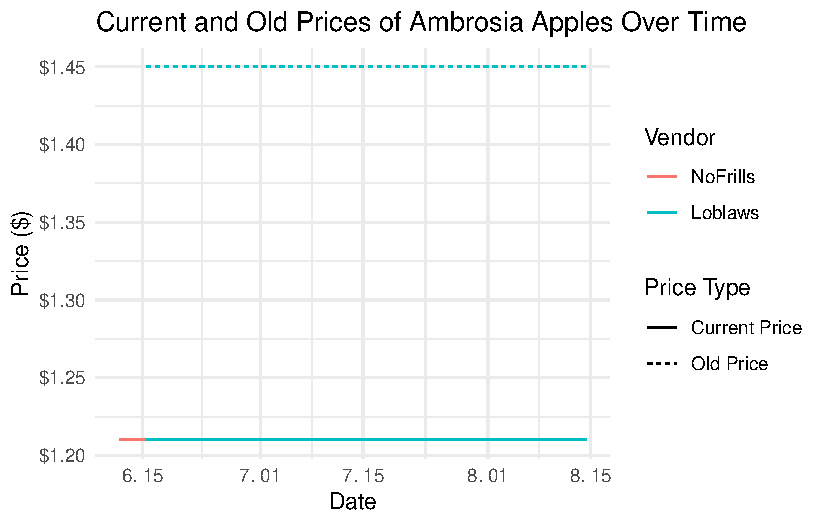
\includegraphics{paper_files/figure-pdf/fig-compare_price_vendor-1.pdf}

}

\caption{\label{fig-compare_price_vendor}Current and Old Prices of
Ambrosia Apples Over Time}

\end{figure}%

We compared the apple prices of nofrills and loblaws at different times
(including the comparison of old prices, where NoFrills does not include
any old prices because this vendor does not have any discounts for this
product and always maintains the original price), which can be seen in
Figure~\ref{fig-compare_price_vendor}.

\subsection{Predictor variables}\label{predictor-variables}

Add graphs, tables and text.

Use sub-sub-headings for each outcome variable and feel free to combine
a few into one if they go together naturally.

\section{Results}\label{results}

Our results are summarized in Table~\ref{tbl-modelresults}.

\begin{table}

\caption{\label{tbl-modelresults}Explanatory models of flight time based
on wing width and wing length}

\centering{

\centering
\begin{tblr}[         %% tabularray outer open
]                     %% tabularray outer close
{                     %% tabularray inner open
colspec={Q[]Q[]},
column{1}={halign=l,},
column{2}={halign=c,},
hline{8}={1,2}{solid, 0.05em, black},
}                     %% tabularray inner close
\toprule
& First model \\ \midrule %% TinyTableHeader
(Intercept) & \num{1.12}    \\
& (\num{1.70})  \\
length      & \num{0.01}    \\
& (\num{0.01})  \\
width       & \num{-0.01}   \\
& (\num{0.02})  \\
Num.Obs.    & \num{19}      \\
R2          & \num{0.320}   \\
R2 Adj.     & \num{0.019}   \\
Log.Lik.    & \num{-18.128} \\
ELPD        & \num{-21.6}   \\
ELPD s.e.   & \num{2.1}     \\
LOOIC       & \num{43.2}    \\
LOOIC s.e.  & \num{4.3}     \\
WAIC        & \num{42.7}    \\
RMSE        & \num{0.60}    \\
\bottomrule
\end{tblr}

}

\end{table}%

\section{Discussion}\label{discussion}

\subsection{First discussion point}\label{sec-first-point}

If my paper were 10 pages, then should be be at least 2.5 pages. The
discussion is a chance to show off what you know and what you learnt
from all this.

\subsection{Second discussion point}\label{second-discussion-point}

Please don't use these as sub-heading labels - change them to be what
your point actually is.

\subsection{Third discussion point}\label{third-discussion-point}

\subsection{Weaknesses and next steps}\label{weaknesses-and-next-steps}

Weaknesses and next steps should also be included.

\newpage

\appendix

\section*{Appendix}\label{appendix}
\addcontentsline{toc}{section}{Appendix}

\section{Additional data details}\label{additional-data-details}

\section{Model details}\label{sec-model-details}

\subsection{Posterior predictive
check}\label{posterior-predictive-check}

In \textbf{?@fig-ppcheckandposteriorvsprior-1} we implement a posterior
predictive check. This shows\ldots{}

In \textbf{?@fig-ppcheckandposteriorvsprior-2} we compare the posterior
with the prior. This shows\ldots{}

\subsection{Diagnostics}\label{diagnostics}

\textbf{?@fig-stanareyouokay-1} is a trace plot. It shows\ldots{} This
suggests\ldots{}

\textbf{?@fig-stanareyouokay-2} is a Rhat plot. It shows\ldots{} This
suggests\ldots{}

\newpage

\section*{References}\label{references}
\addcontentsline{toc}{section}{References}

\phantomsection\label{refs}
\begin{CSLReferences}{1}{0}
\bibitem[\citeproctext]{ref-tellingstories}
Alexander, Rohan. 2023. \emph{Telling Stories with Data}. Chapman;
Hall/CRC. \url{https://tellingstorieswithdata.com/}.

\bibitem[\citeproctext]{ref-citeR}
R Core Team. 2023. \emph{{R: A Language and Environment for Statistical
Computing}}. Vienna, Austria: R Foundation for Statistical Computing.
\url{https://www.R-project.org/}.

\end{CSLReferences}




\end{document}
